Acts stands for \textit{a common tracking software} and is a community-driven project that aims to provide experiment independent track reconstruction algorithms written in modern C++ \cite{acts-2022}. Its origins are close to the ATLAS track reconstruction software, and the majority of its main developers are members of the ATLAS collaboration to this day. Acts is planned to be used extensively in the ATLAS Phase-2 reconstruction and potentially fast track simulation \cite{atlas-tdr-029-add}. Apart from that, it is already adopted or in the process of adaptation by various other experiments, such as: Faser \cite{faser}\cite{faser2}, sPHENIX \cite{sphenix}, STCF \cite{stcf}, LDMX \cite{ldmx}, ePIC \cite{epic}, Alice \cite{alice}, COMET \cite{comet2}, NA60+ \cite{na60+}, Lohengrin \cite{lohengrin}, and CEPC \cite{cepc}. The project is open source and can be found on GitHub \footnote{\url{https://github.com/acts-project/acts}}.

% Acts is structured in a modular way, where each component is responsible for a specific task. Examples are: the magnetic field, material, geometry, propagation, track finding, track fitting, and vertexing. These components interact with each other in various ways.

Acts consists of two main parts: the Core library and the Examples framework. The Core library is a toolbox and meant to be used by an experiments' reconstruction framework. The Examples framework demonstrates how to use the Core library and allows to run algorithms on simulated detectors. It can be used for educational purposes, testing and early performance studies. It is generally disencouraged to use the Examples framework for production workflows.

The reason for this separation is that a reconstruction framework is highly experiment specific and should be tailored to the needs of the experiment. The Core library is meant to be used as a building block for such a framework. The Examples framework can also be thought of as a starting point for new users to get familiar with the Core library.

This chapter gives a brief overview of the Acts project and reviews the core concepts and definitions. First, core components and their connections are described. Followed by definitions and choices for units, constants, track parameterization and event data model. Then, the tracking geometry and Fatras, the fast track simulation module, are introduced. Followed by an introduction to the Examples framework and the OpenDataDetector.

\section{Components and their connections}

Acts can be thought of as a collection of components which interact with each other to build higher and higher levels of abstractions. The most basic building blocks are the magnetic field, the geometry and the material. The magnetic field can be queried for its field strength at a given point in space. There are a few implementations available with the simplest one being a constant field. The geometry component deals with surfaces, layers and volumes which built up the tracking geometry of a detector. The material component abstracts material properties and provides utilities to estimate interactions like ionization loss and multiple scattering for a given incident particle.

The propagator component is responsible for moving parameters along a particle's trajectory. The most prominent use case is to extrapolate track parameters from one surface to another. The propagator uses the magnetic field to estimate the beding of the particle's trajectory. The geometry is used to check for intersections with the tracking geometry and the material is used to estimate energy loss and multiple scattering.

Ultimately, algorithms are built on top of these components. Some of them depend on the propagation, like classical track finding and track fitting algorithms, while others just depend on the geometry, like the spacepoint formation.

There are a few more definitions and concepts which do not necessarily map directly to single components in the code. Two of these are units and constants, and the track parameterization, which are discussed in the following sections.

\section{Units and constants}

Acts uses a defined set of relevant units to make sense of physical quantities. They can be found in \texttt{Acts/Definitions/Units.hpp}.

Most importantly, lengths are measured in millimeters and energies in GeV. The speed of light is set to 1, which implicitly sets the time unit to millimeters. Time in seconds can be obtained by dividing the quantity with pre-defined constants which are related to the SI units.

Units are ultimately a choice, but one that is taken by Acts and not the user. Having a consistent, pre-defined set of units allows for easier to read and consistent code. The types of scalars and vectors in Acts do not reflect their units, since they are implicit for the dimension. Some decisions taken for units and constants reach further into the Acts codebase than just \texttt{Units.hpp}. For example $c = 1$ is built implicitly into many equations.

The choice of measuring length in millimeters has direct consequences for the time units. The distance light travels in one nanosecond in vacuum $1\ \text{ns} = 299.79\ \text{mm/c}$ results in a big value compared to the typical spatial resolution of micrometers in tracking detectors. This can potentially lead to numerical instabilities and may need reconsideration in the future.

\section{Track parameterization}
\label{sec:intro/acts/track-parameterization}

Track parameters describe the observable state of a track at a given point in space and/or time. This includes the position, time, direction, and charge over momentum. There are two kinds of track parameters in Acts: bound parameters and free parameters. Bound track parameters are expressed with a local position at a given surface, a direction with two spherical coordinate angles, while free track parameters are expressed with a global cartesian position and a normalized direction vector.

\begin{equation}
    \mathbf{x}_\text{local} = \left(l_0, l_1, \phi, \theta, q/p, t\right)^\mathrm{T}
\end{equation}

\begin{equation}
    \mathbf{x}_\text{global} = \left(g_0, g_1, g_2, t, d_0, d_1, d_2, q/p\right)^\mathrm{T}
\end{equation}

The azimuthal angle, $\phi$, should be within $[-\pi, \pi)$, but values outside this range are also accepted as they uniquely map to a valid value in the range. The polar angle, $\theta$, has to be within $[0, \pi]$, while $0$ and $\pi$ should be avoided as they correspond to the poles of the spherical coordinate system. The charge over momentum parameter, $q/p$, captures the curvature of the trajectory given the local magnetic field. This choice can be motivated by the equations of motion for a free particle in a magnetic field. The charge is signed and the momentum is the magnitude of the momentum vector. Using the absolute momentum magnitude over the traverse momentum magnitude is more general given an arbitraty magnetic field. To extract the momentum from $q/p$, one has to assume an absolute charge of the particle.

In Acts, \texttt{BoundTrackParameters} contain the bound parameter vector, the surface, a particle hypothesis and optionally a covariance matrix. Similarly, \texttt{FreeTrackParameters} contain the free parameter vector, a particle hypothesis and optionally a covariance matrix.

Note that the Acts \texttt{BoundTrackParameters} are sort of standard for collider experiments. This comes with two caveats: the bound parametrization does not make a lot of sense for foward exteriments and there are poles in the parametrization which can lead to numerical instabilities. This can be avoided by rotating the tracking geometry away from the poles.

Track parametrization is ultimately a choice and there is not single best one. Since Acts aims to be experiment independent, a more general solution would be preferable but was not reached yet. The parametrization is deeply baked into Acts which makes it hard to change. At the same time an abstraction for the track parameters might bring a compute performance penalty.

% Track parameters should be unique and "well-behaved" in the sense that they should not have singularities or discontinuities. This is not always the case with the Acts track parameters. Additionally, for numerical stability, they should live on a similar scale which also depends on the units and geometry.

\section{Event data model}

The event data model (EDM) in Acts is a collection of data structures which are used to store inputs and outputs of the reconstruction. For example, Acts Core defines containers and access to spacepoints, seeds and tracks. While Acts Examples defines remaining types like clusters and measurements. Current EDM implementations try to be experiment independent by defining interfaces for read and write access and providing default implementations within Acts Core. The main reason for this is to avoid copying data to and from user-defined data structures. This is beneficial for memory usage, but might have performance implications which are currently under investigation. Potentially Acts could define a set of EDM types and couple its algorithms to these types directly. This would also avoid C++ template interfaces in the algorihtms.

Most tracking EDMs can be thought of as tables. Each row corresponds to a single object and each column corresponds to a property of the object. The rows are indexed by an integer ID which is unique for the object. An example for this is the track EDM. The track container stores track parameters, the reference surface, the particle hypothesis and the last track state index which points into the track state container. The track state container stores track parameters for each surface crossed and links to the previous track states.

\section{Tracking geometry}

A tracking geometry is a simplified version of the full detector geometry with the purpose of simplifying and accelerating tracking algorithms. Real detectors consist of support structures, cables, cooling pipes, etc. which are not directly relevant for track reconstruction algorithms. The Acts tracking geometry consists of surfaces, layers, and volumes. These are hierarchical: volumes contain layers, and layers contain surfaces. Surfaces come in different shapes, like rectangular or cylindrical. Volumes are enclosed with boundary surfaces, which connect to other volumes or to the end of world.

The tracking geometry distinguishes between sensitive and passive surfaces. Sensitive surfaces measure parts of the state or properties of particles, like their 2D hit position. Passive surfaces represent logical structures of the detector or carry accumulated passive detector material. The procedure of deriving this accumulated material is called \textit{material mapping}.

\begin{figure}[H]
    \centering
    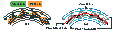
\includegraphics[width=1.0\textwidth]{parts/1_introduction/03_acts-introduction/figures/tracking_geometry.pdf}
    \caption{Illustration of (a) a detector geometry with sensitive parts in green and passive parts in orange and (b) a corresponding tracking geometry. Gracefully taken from \textcite{gessinger-thesis}.}
    \label{fig:intro/acts/tracking-geometry}
\end{figure}

Figure \ref{fig:intro/acts/tracking-geometry} illustrates the difference between a detector geometry and tracking geometry. Apart from the simplification of passive detector parts, the geometry is grouped into logical components. A cylindrical volume captures the layer which contains the sensitive surfaces. The layer is represented by a cylinder surface and enclosed by two approach surfaces. The approach surfaces are special passive surface which guide the navigation towards sensitive surfaces.

\section{Fatras}
\label{sec:intro/acts/fatras}

Acts comes with a fast track simulation module called Fatras. It can be used to simulate the passage of particles through a detector based on its tracking geometry, magnetic field and mapped material.

Fatras is heavily used in Acts Examples, for testing Acts in general, and early performance studies. The main benefit is its speed compared to full simulation frameworks like Geant4 \cite{geant4-2003}\cite{geant4-2006}\cite{geant4-2016}, and its simplicity by directly using the Acts geometry and material. Fatras is not meant to be used for detailed studies as it only implementes a few physics interactions but for instance no hadronic interactions.

\section{Plugins}

Acts comes with a list of plugins which can be used to extend the functionality of the Core library with additional external dependencies. Acts Core is designed to have a minimal set of dependencies. Everything that goes beyond these are optional and captured by a plugin. Plugins can be enabled or disabled during the build process.

There are geometry plugins to deal with different input sources like DD4hep \cite{dd4hep}, GeoModel \cite{geomodel}, ROOT's TGeo \cite{root}, and Geant4. There are also plugins for serialization and deserialization of data like Json, EDM4hep \cite{edm4hep}, and ROOT.

\section{The Examples framework}

The Examples framework exercises the use of the Core library to build a reconstruction framework. It can be used for educational purposes, testing and early performance studies. At the same time it serves as a starting point for new users to get familiar with the Core library. It is generally discouraged to use it for production workflows. As such, the Examples are not subject to the same level of scrutiny as the Core library.

The goal of the Examples is to test common workflows and to enable monitoring of our algorithms on a higher level. Testing within the Core library cannot include a detailed simulation and reconstruction chains. The Examples framework provides a way to test the Core library in a more realistic environment.

The Examples provide various detectors, such as a generic telescope detector and the OpenDataDetector. A sequencer component allows to execute reconstruction algorihtms in a given order. There is a central event data store called \texttt{Whiteboard}, which can be used by algorithms to reach for their input and return their output to. Algorithms perform the individual steps of the reconstruction chain, like track finding, track fitting, and vertexing. Readers and writers can be used to move event and reconstruction data from and to disk. Special summary writers exist to measure the performance of reconstruction algorithms using truth information.

\section{The OpenDataDetector}

The OpenDataDetector (ODD) \cite{odd-v2} is an evolution of the TrackML \cite{trackml} detector with a more realistic material budget and simulation support with Geant4. It is an (HL-)LHC-like full silicon prototype inner detector based on DD4hep and consists of 3 sub detectors: Pixel, Short Strips, and Long Strips. Since recently, the ODD can be extended with calorimeters \cite{odd-chep} and a muon system, to investigate other reconstruction techniques. The layout of the ODD inner tracking system is illustrated in Figure \ref{fig:intro/acts/odd-layout}. The Long Strips are two sided modules rotated with a stereo angle of 4 mrad. Details about the sub detectors are summaried in Table \ref{tab:intro/acts/odd-details}. The project is open source and can be found on CERN's GitLab instance \footnote{\url{https://gitlab.cern.ch/acts/OpenDataDetector}}.

\begin{figure}[H]
    \centering
    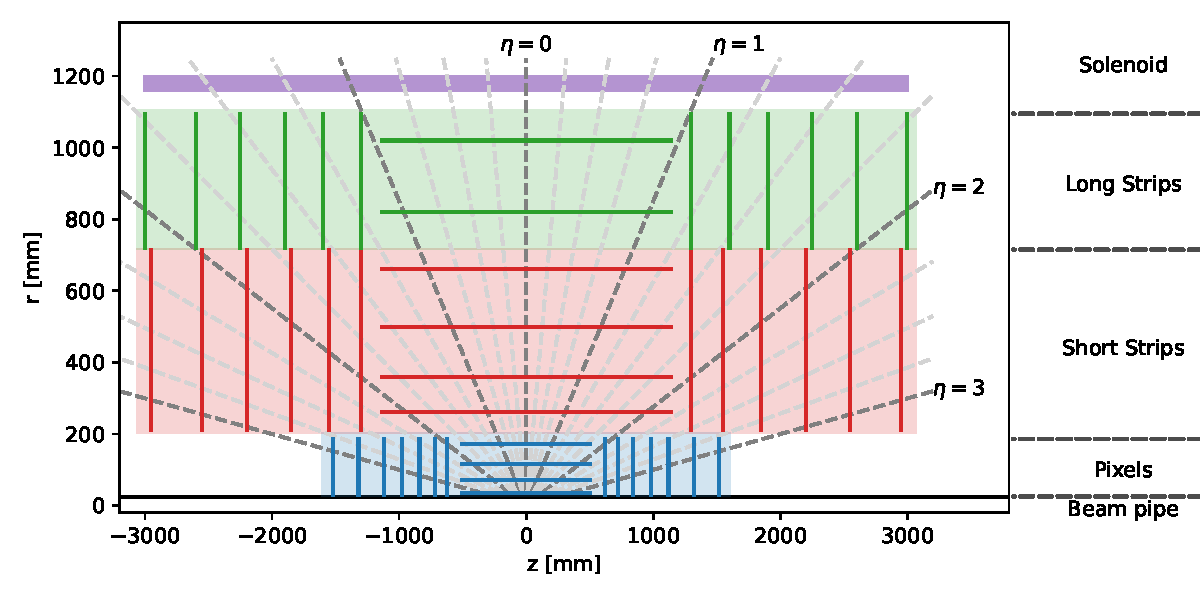
\includegraphics[width=1.0\textwidth]{parts/1_introduction/03_acts-introduction/figures/odd_layout.pdf}
    \caption{Illustration of the ODD layout from a Z-R view, segmented into: Beam pip, Pixels, Short Strips, Long Strips, and Solenoid. The solid lines inside the sub detectors represent the layers. The dashed lines represent different eta regions.}
    \label{fig:intro/acts/odd-layout}
\end{figure}

\begin{table}[H]
    \centering
    \begin{tabular}{c|c|c|c}
       \textbf{Sub detector} & \textbf{Measurement} & \textbf{Resolution} & \begin{tabular}{c}\textbf{Layers barrel /}\\\textbf{endcap}\end{tabular} \\
       \hline
       Pixel & \begin{tabular}{c}2D + time\end{tabular} & \begin{tabular}{c}15 µm spatial\\25 mm/c temporal\end{tabular} & 4 / 7 \\
       \hline
       Short Strip & 2D & \begin{tabular}{c}43 µm spatial x\\1.2 mm spatial y\end{tabular} & 4 / 6 \\
       \hline
       Long Strip & 1D & 72 µm spatial & 2 / 6 \\
    \end{tabular}
    \caption{Details about the ODD sub detectors. Note that spatial and temporal resolutions are configurable. But they are consistently used as provided here in an Acts context.}
    \label{tab:intro/acts/odd-details}
\end{table}

Acts Examples uses DD4hep to construct a tracking geometry from the detector description of the ODD. This geometry can then be used for track reconstruction and fast track simulation (Fatras). A more realistic simulation can be achieved using Geant4. Events can be generated using a particle gun or Pythia8 \cite{pythia8}.

The reference frame used for the ODD is defined as follows: the Z axis points along the beam line, the Y axis points towards the center of an imaginary accelerator, and the X axis is determined by the right hand rule. The azimuthal angle $\phi$ is defined as $\phi = \text{atan2}(y,x)$ in the transverse plane XY, and the polar angle $\theta$ is defined as $\theta = \text{atan2}(\sqrt{x^2+y^2},z)$. The pseudo rapidity $\eta$ is given by $\eta = -\text{ln}(\text{tan}\frac{\theta}{2})$.

\begin{figure}[H]
    \centering
    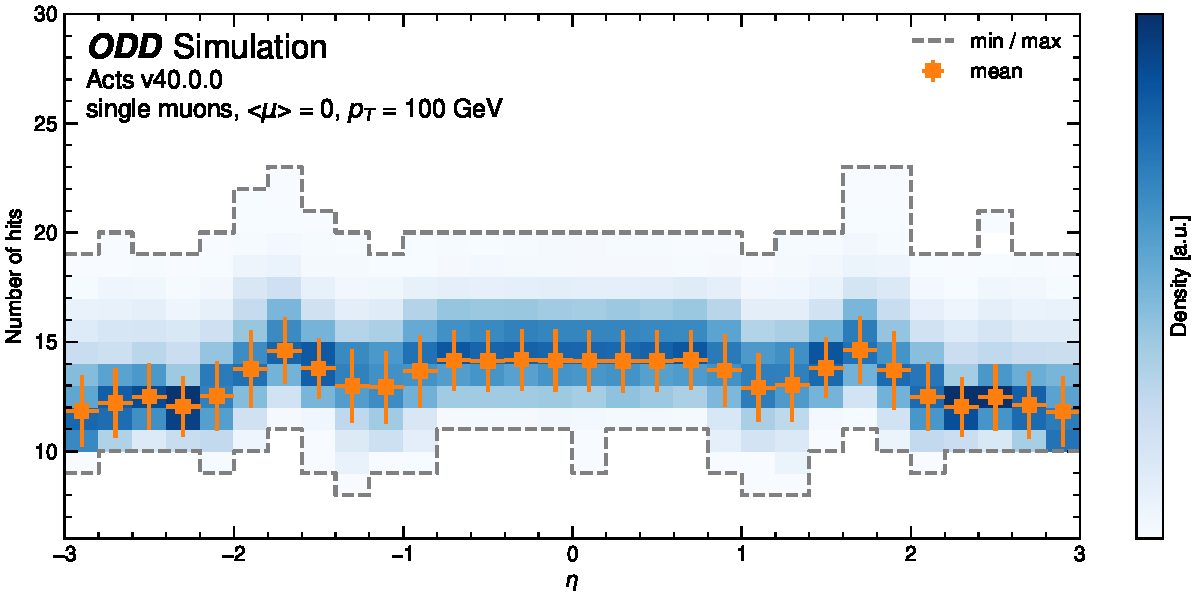
\includegraphics[width=1.0\textwidth]{parts/1_introduction/03_acts-introduction/figures/odd_hits.pdf}
    \caption{Number of hits as a function of $\eta$ for single $\mu$ with $p_T = 100$ GeV. The dashed lines indicate the minimum and maximum number of hits per $\eta$ bin.}
    \label{fig:intro/acts/odd-hits}
\end{figure}

Figure \ref{fig:intro/acts/odd-hits} shows the number of hits as a function of $\eta$ for single muons with $p_T = 100$ GeV. For the majority of particles, 10 or more hits are produced, with an average of 14 in the barrel region $|\eta| < 1$.

\begin{figure}[H]
    \centering
    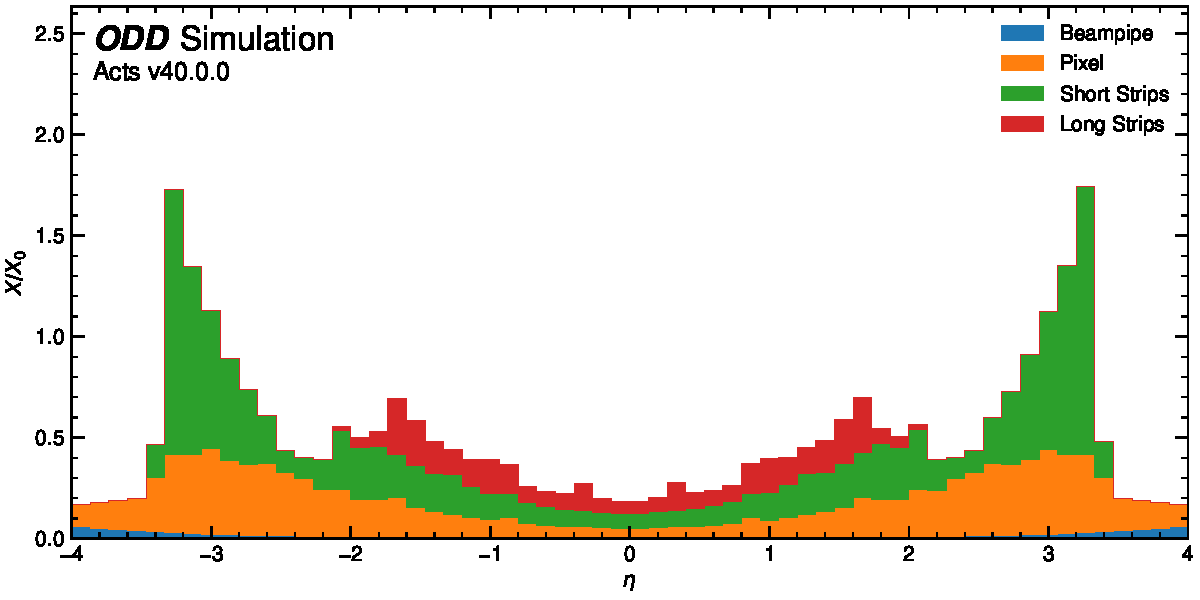
\includegraphics[width=1.0\textwidth]{parts/1_introduction/03_acts-introduction/figures/odd_material_x0_eta.pdf}
    \caption{Material amount in $X/X_0$ as a function of $\eta$. The vertical dashed lines indicate the usual $[-3,3]$ $\eta$ coverage.}
    \label{fig:intro/acts/odd-material-x0-eta}
\end{figure}

Figure \ref{fig:intro/acts/odd-material-x0-eta} shows the amount of material in $X/X_0$ as a function of $\eta$. The material amount is sampled with Geant4. The number of crossed radiation lengths $X/X_0$ determines the amount of energy loss and multiple scattering a particle experiences while traversing the detector. The material amount is not constant and varies with $\eta$ due to geometric effects. $X/X_0$ determines the impact parameter resolution of the detector.

\begin{figure}[H]
    \centering
    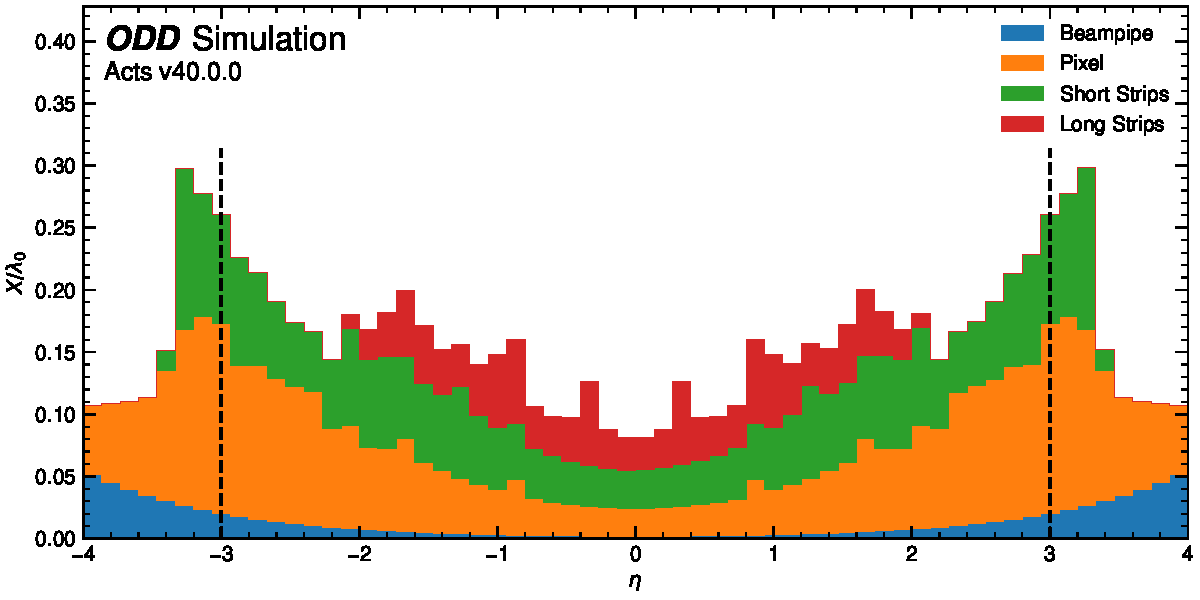
\includegraphics[width=1.0\textwidth]{parts/1_introduction/03_acts-introduction/figures/odd_material_l0_eta.pdf}
    \caption{Material amount in $X/\lambda_0$ as a function of $\eta$. The vertical dashed lines indicate the usual $[-3,3]$ $\eta$ coverage.}
    \label{fig:intro/acts/odd-material-l0-eta}
\end{figure}

Figure \ref{fig:intro/acts/odd-material-l0-eta} shows the amount of material in $X/\lambda_0$ as a function of $\eta$. The number of crossed nuclear interaction lengths $X/\lambda_0$ determines the number of nuclear interactions a hadron experiences on average while traversing the detector. As such, $X/\lambda_0$ also determines the upper bound of efficiency for hadrons.
